
%%%%%%%%%%%%%%%%%%%%%%%%%%%%%%%%%%%%%%%%%%%%%%%%%%%%%%%%%%%%%%%%%%%%%%%%
\chapter{Semantics of the \fnamee Calculus}
\label{chap:fi}
%%%%%%%%%%%%%%%%%%%%%%%%%%%%%%%%%%%%%%%%%%%%%%%%%%%%%%%%%%%%%%%%%%%%%%%%

In this chapter, we present \fnamee, the first typed calculus combining disjoint
polymorphism with BCD subtyping. \fnamee is essentially a hybrid of \namee
(which does not support parametric polymorphism) and \fname (which does not
account for BCD subtyping). As we will see, the combination is very expressive,
enabling improved compositional designs and supporting automated composition of
interpretations in programming techniques like object
algebras~\citep{oliveira2012extensibility} and finally
tagless~\citep{CARETTE_2009}. Furthermore, as we will show in
\cref{chap:traits}, \fnamee is able to encode sophisticated concepts such as
mixins/traits and dynamic inheritance. Unfortunately, the combination also
introduces non-trivial complications. The main technical challenge (like for
most other calculi with disjoint intersection types) is the proof of
coherence---our main topic in \cref{chap:coherence:poly}.


The formalization and metatheory of \fnamee are a significant advance over its
predecessor \fname. Besides the support for distributive subtyping, \fnamee
removes several restrictions imposed by the syntactic coherence proof in \fname.
In particular \fnamee supports unrestricted intersections, which are forbidden
in \fname. Unrestricted intersections enable, for example, encoding certain
forms of bounded quantification~\citep{pierce1991programming}. Moreover the new
proof method is more robust with respect to language extensions. For instance,
\fnamee supports the bottom type without significant complications in the
proofs, while it was a challenging open problem in \fname. A final interesting
aspect is that \fnamee's type-checking is decidable. In the design space of
languages with polymorphism and subtyping, similar mechanisms have been known to
lead to undecidability. Pierce's seminal paper ``\emph{Bounded quantification is
  undecidable}''~\citep{pierce1994bounded} shows that the contravariant subtyping
rule for bounded quantification in \fsub leads to undecidability of subtyping.
In \fnamee the contravariant rule for disjoint quantification retains
decidability. Since with unrestricted intersections \fnamee can express several
use cases of bounded quantification, \fnamee could be an interesting and
decidable alternative to \fsub.



\section{\namee by Examples}
\label{nested:sec:overview}

This section illustrates \namee with an encoding of a family polymorphism
solution to the expression problem, and informally presents its salient
features.


%-------------------------------------------------------------------------------
\subsection{The Expression Problem, \namee Style}

The \namee calculus allows us to solve the expression problem in a way that is
very similar to \citeauthor{Ernst_2001}'s \textsf{gbeta} solution in \cref{sec:ernst}.
However, the underlying mechanisms of \namee are quite different from those of
\textsf{gbeta}. In particular, \namee features a structural type system in which we can
model objects with records, and object types with record types. For instance, we
model the interface of \lstinline{Lang.Exp} with the singleton record type
\lstinline${ print : String }$. For the sake of conciseness, we use \lstinline{type} aliases
to abbreviate types.
\lstinputlisting[linerange=4-4]{./examples/overview.sl}% APPLY:linerange=PRINT_INTERFACE
Similarly, we capture the interface of the \lstinline{Lang} family in a record,
with one field for each case's constructor.
\lstinputlisting[linerange=8-8]{./examples/overview.sl}% APPLY:linerange=LANG_FAMILY
Here is the implementation of \lstinline{Lang}.
\lstinputlisting[linerange=17-24]{./examples/overview.sl}% APPLY:linerange=LANG_IMPL
We assume several primitive types: fixed width integers \lstinline{Int},
\lstinline{Double} for numeric operations and \lstinline{String} for text
manipulation. A \namee program consists of a collection of definitions and
declarations, separated by semicolon \lstinline{;}.

% - - - - - - - - - - - - - - - - - - - - - - - - - - - - - - - - - - - - - - - -
\paragraph{Adding evaluation.}
We obtain \lstinline{IPrint & IEval}, which is the corresponding type for \lstinline{LangEval.Exp}, by
intersecting \lstinline{IPrint} with \lstinline{IEval} where
\lstinputlisting[linerange=29-29]{./examples/overview.sl}% APPLY:linerange=EVAL_INTERFACE
The type for \lstinline{LangEval} is then
\lstinputlisting[linerange=34-37]{./examples/overview.sl}% APPLY:linerange=EVAL_PRINT_INTERFACE
We obtain an implementation for \lstinline{LangEval} by merging the existing
\lstinline{Lang} implementation \lstinline{implLang} with the new evaluation
functionality \lstinline{implEval} using the merge operator \lstinline{,,}.
\lstinputlisting[linerange=45-53]{./examples/overview.sl}% APPLY:linerange=EVAL_PRINT_IMPL

% - - - - - - - - - - - - - - - - - - - - - - - - - - - - - - - - - - - - - - - -
\paragraph{Adding negation.}
Adding negation to \lstinline{Lang} works similarly.
\lstinputlisting[linerange=57-65]{./examples/overview.sl}% APPLY:linerange=LANG_NEG
% \begin{Verbatim}[xleftmargin=10mm,fontsize=\relscale{.80}]
% type LangNeg = Lang & { neg : IPrint -> IPrint }

% implLangNeg : LangNeg
% implLangNeg = implLang ,, implNeg

% implNeg = { neg = \a.{print = "-" ++ a.print } }
% \end{Verbatim}

% - - - - - - - - - - - - - - - - - - - - - - - - - - - - - - - - - - - - - - - -
\paragraph{Putting everything together.}
Finally, we can combine the two extensions and provide the missing
implementation of evaluation for the negation case.
\lstinputlisting[linerange=70-80]{./examples/overview.sl}% APPLY:linerange=LANG_FINAL
We can test \lstinline{implLangNegEval} by creating an object that represents $-2 + 3$, which is able to print and evaluate at the same time.
\lstinputlisting[linerange=98-100]{./examples/overview.sl}% APPLY:linerange=TEST



%- - - - - - - - - - - - - - - - - - - - - - - - - - - - - - - - - - - - - - - -
\paragraph{Multi-field records.}
Recall that in \cref{bg:sec:intersection}, we show how to model multi-field records by
single-field records. Thus \namee does not have multi-field record types built in.
They are merely syntactic sugar for intersections of single-field record types.
Hence, the following is an equivalent definition of \lstinline{Lang}:
\lstinputlisting[linerange=13-13]{./examples/overview.sl}% APPLY:linerange=LANG_FAMILY2
Similarly, the multi-field record expression in the definition of
\lstinline{implLang} is syntactic sugar for the explicit merge of two
single-field records.
\begin{lstlisting}
implLang : Lang = { lit = ... } ,, { add = ... };
\end{lstlisting}

%- - - - - - - - - - - - - - - - - - - - - - - - - - - - - - - - - - - - - - - -
\paragraph{Subtyping.}
A distinctive difference compared to \textsf{gbeta} is that many more \namee types are related through
subtyping. Indeed, \textsf{gbeta} is unnecessarily conservative~\citep{ernst_hoh}: none of the families is related
through subtyping, nor is any of the class members of one family related to any
of the class members in another family. For instance, \lstinline{LangEval} is
not a subtype of \lstinline{Lang}, nor is \lstinline{LangNeg.Lit} a subtype
of \lstinline{Lang.Lit}.

In contrast, subtyping in \namee is much more nuanced and depends entirely on the
structure of types. The primary source of subtyping are intersection types:
any intersection type is a subtype of its components. For instance, 
\lstinline{IPrint & IEval} is a subtype of both \lstinline{IPrint} and
\lstinline{IEval}. Similarly \lstinline{LangNeg = Lang & NegPrint} is a subtype
of \lstinline{Lang}. Compare this to \textsf{gbeta} where \lstinline{LangEval.Expr} is
not a subtype of \lstinline{Lang.Expr}, nor is the family \lstinline{LangNeg} a
subtype of the family \lstinline{Lang}.

However, \textsf{gbeta} and \namee agree that \lstinline{LangEval} is not a subtype of
\lstinline{Lang}. The \namee-side of this may seem contradictory at first, as we
have seen that intersection types arise from the use of the merge operator.
We have created an implementation for \lstinline{LangEval} with
\lstinline{implLang ,, implEval} where \lstinline{implLang} has type \lstinline{Lang}, which
suggests that \lstinline{LangEval} is a subtype of \lstinline{Lang}.
Yet, there is a flaw in our reasoning:
strictly speaking, \lstinline{implLang ,, implEval} is not of
type \lstinline{LangEval} but instead of type \lstinline{Lang & EvalExt}, where
\lstinline{EvalExt} is the type of \lstinline{implEval}:
\lstinputlisting[linerange=41-41]{./examples/overview.sl}% APPLY:linerange=EVAL_INTERFACE2

Nevertheless, the definition of \lstinline{implLangEval} is valid because
\lstinline{Lang & EvalExt} is a subtype of \lstinline{LangEval}.
Indeed, if we consider for the sake of simplicity only the \lstinline{lit}
field, we have that \lstinline{(Int -> IPrint) & (Int -> IEval)} is a
subtype of \lstinline{Int -> IPrint & IEval}. This follows from a standard
subtyping axiom for distributivity of functions and intersections in the BCD system inherited by \namee.
In conclusion, \lstinline{Lang & EvalExt} is a subtype of both \lstinline{Lang}
and of \lstinline{LangEval}. However, neither of the latter two types is a subtype of the other.
Indeed, \lstinline{LangEval} is not a subtype of \lstinline{Lang} as the type
of \lstinline{add} is not covariantly refined and thus admitting the subtyping
is unsound. For the same reason \lstinline{Lang} is not a subtype of \lstinline{LangEval}.


A summary of the various relationships between the language components is shown
in \cref{fig:diagram}. Admittedly, the figure looks quite complex because our
calculus has a structural type system (as often more foundational calculi
do) where more types are related through subtyping, whereas mainstream object-oriented
languages have nominal type systems.



\begin{figure}[t]
  \centering
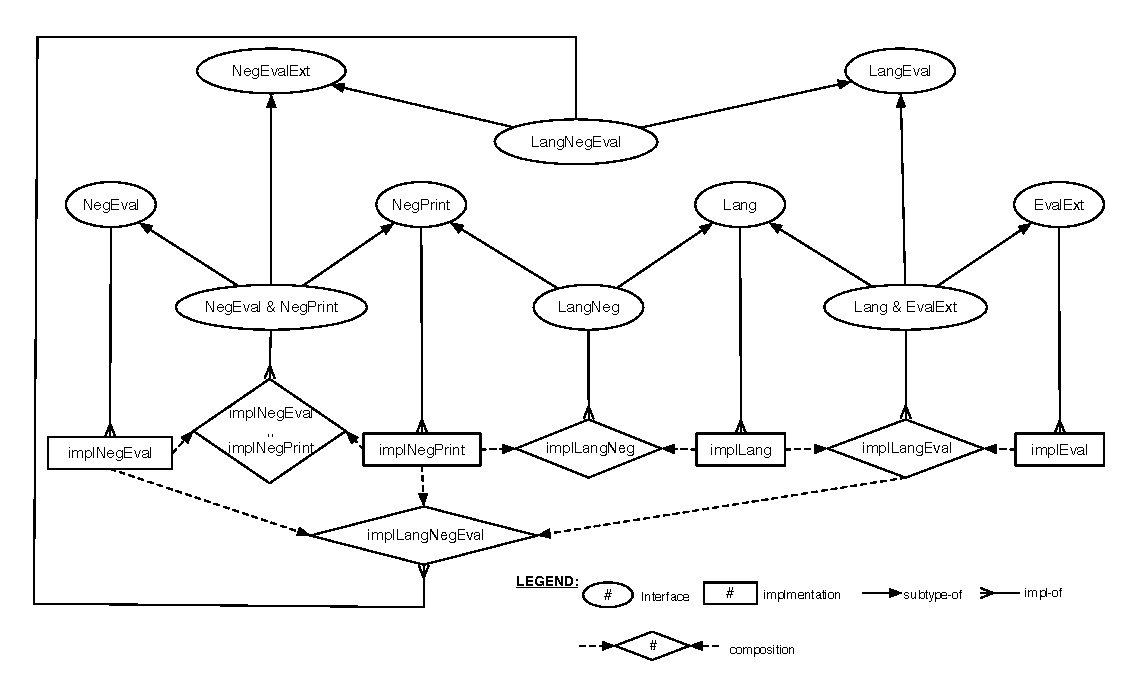
\includegraphics[scale=0.75]{figures/diagram.eps}
\caption{Summary of the relationships between language components}
\label{fig:diagram}
\end{figure}


\paragraph{Stand-alone extensions.}
Unlike in \textsf{gbeta} and other class-based inheritance systems, in \namee
the extension \lstinline{implEval} is not tied to \lstinline{LangEval}. In that
sense, it resembles trait and mixin systems that can apply the same extension
to different classes. However, unlike those systems, \lstinline{implEval} can also
exist as a value on its own, i.e., it is not an extension per se.

%-------------------------------------------------------------------------------
% \subsection{Disjoint Intersection Types and Ambiguity}

% The above example shows that intersection types and the merge operator
% are closely related to multiple
% inheritance. Indeed, they share a major concern with multiple inheritance,
% namely ambiguity. When a subclass inherits an implementation of the same
% method from two different parent classes, it is unclear which of the two
% methods is to be adopted by the subclass. In the case where the two parent classes
% have a common superclass, this is known as the \emph{diamond problem}.
% The ambiguity problem also appears in \namee,
% e.g., if we merge two numbers to obtain $\mer{1}{2}$ of type
% $\inter{\mathsf{Int}}{\mathsf{Int}}$. Is the result of $\mer{1}{2} + 3$
% either $4$ or $5$?

% Disjoint intersection types offer to statically detect potential ambiguity and
% to ask the programmer to explicitly resolve the ambiguity by rejecting the
% program in its ambiguous form. In the previous work on \oname, ambiguity is
% avoided by dictating that all intersection types have to be disjoint, i.e.,
% $\inter{\mathsf{Int}}{\mathsf{Int}}$ is ill-formed because the first component
% has the same type as the second.


% Disjoint intersection types ensure unambiguity and conflicts are
% statically detected and manually resolved by programmers. This
% is similar to the trait model.


% Local Variables:
% TeX-master: "../../Thesis"
% org-ref-default-bibliography: ../../Thesis.bib
% End:


\section{Syntax and Semantics}

\begin{figure}[t]
  \centering
\begin{tabular}{llll} \toprule
  Types & $[[A]], [[B]], [[C]]$ & $\Coloneqq$ & $[[nat]] \mid [[Top]] \mid [[A -> B]]  \mid [[A & B]] \mid [[{l : A}]] \mid [[X]] \mid [[\ X ** A . B]] $\\
  Monotypes & $[[t]]$ & $\Coloneqq$ & $[[nat]] \mid [[Top]] \mid [[t1 -> t2]]  \mid [[t1 & t2]] \mid [[X]] \mid [[{l : t}]]$\\
  Expressions & $[[ee]]$ & $\Coloneqq$ & $[[x]] \mid [[i]] \mid [[Top]] \mid [[\x . ee]] \mid [[ee1 ee2]] \mid [[ ee1 ,, ee2 ]]   \mid [[ ee : A ]] $ \\
        & & $\mid$ & $ [[{l = ee}]] \mid [[ ee.l  ]] \mid [[\X ** A . ee]] \mid [[ ee A ]]  $ \\
  Value Contexts & $[[GG]]$ & $\Coloneqq$ &  $[[empty]] \mid [[GG , x : A]] $ \\
  Type Contexts & $[[DD]]$ & $\Coloneqq$ &  $[[empty]] \mid [[DD , X ** A]] $  \\ \bottomrule
  % Expression Contexts & $[[CC]]$ & $\Coloneqq$ &  $[[__]] \mid [[\ x . CC]] \mid [[\ X ** A. CC]] \mid [[ CC A  ]] \mid [[CC ee]] \mid [[ee CC]] \mid [[ CC ,, ee  ]]  $ \\
  % & & $\mid$ & $[[ ee ,, CC  ]] \mid  [[ { l = CC}  ]]  \mid [[ CC . l]] $
\end{tabular}
  \caption{Syntax of \fnamee}
  \label{fig:syntax:fi}
\end{figure}

\Cref{fig:syntax:fi} shows the syntax of \fnamee. Metavariables $[[A]], [[B]],
[[C]]$ range over types. Apart from \namee types, \fnamee also includes type
variables $[[X]]$ and disjoint quantification $[[ \X ** A . B ]]$. Monotypes
$[[t]]$ are the same, less the universal quantification. Metavariable $[[ee]]$
ranges over expressions. We extend \namee expressions with two standard
constructs in System F: type abstractions $[[ \X ** A . ee ]]$ and type
applications $[[ee A]]$. The former also includes an extra disjointness
constraint $[[A]]$ associated with the type variable $[[X]]$.

\paragraph{Contexts.}

In the traditional formulation of System F, there is a single context that is
used to keep track of both type variables and term variables. Here we use
another style of presentation~\citep[chap. 16]{Harper_2016} where contexts are
split into \textit{value contexts} $[[GG]]$ and \textit{type contexts} $[[DD]]$.
The former track bound term variables $[[x]]$ with their types $[[A]]$; and the
latter track bound type variables $[[X]]$ with their disjointness constraints
$[[A]]$. This formulation is also convenient for the presentation of logical
relations in \cref{chap:coherence:poly}.

\begin{figure}
  \centering
  \drules[swft]{$[[DD |- A]]$}{Well-formedness of types}{top, int, var, arrow, all, and, rcd}
  \drules[swfe]{$[[DD ||- GG]]$}{Well-formedness of value contexts}{empty, var}
  \drules[swfte]{$[[||- DD]]$}{Well-formedness of type contexts}{empty, var}
  \caption{Well-formedness of contexts and types}
  \label{fig:well-formedness:fi}
\end{figure}

\paragraph{Well-formedness of contexts.}

The well-formedness judgments for contexts and types, as shown in
\cref{fig:well-formedness:fi} are quite standard. They together ensure that each
type appearing in the contexts is well-formed in the sense that there are no
unbound free variables.


\paragraph{Declarative Subtyping.}


\begin{figure}[h]
  \centering
  \drules[FS]{$[[ A <|: B ~~> c]]$}{Declarative subtyping}{refl,trans,top,rcd, arr,andr,andl,and,distArr,topArr,distRcd,topRcd,forall}
  \caption{Declarative subtyping of \fnamee}
  \label{fig:subtyping:fi}
\end{figure}

\Cref{fig:subtyping:fi} presents the subtyping relation of \fnamee. For now, we
ignore the coercion parts ($[[~~>]] [[c]]$) and explain them in
\cref{sec:elaboration:fi}. We naturally extend the subtyping rules of \namee
with only one rule \rref*{FS-forall}, which specifies the subtyping relation
between two universal quantifiers. In \rref{FS-forall}, a universal quantifier
is covariant in its body, and contravariant in its disjointness constraint. A
minor comment is that since \fnamee features explicit polymorphism, type
variables are neutral to subtyping, i.e., $[[X <: X]]$, which is contained in
\rref{FS-refl}. As with \namee subtyping, the subtyping relation of \fnamee is
trivially \textit{reflexive} and \textit{transitive}.

\begin{remark}
  In our Coq formalization, we require that the two types $[[A]]$ and $[[B]]$ are
  well-formed with respect to some type context, resulting in the subtyping
  judgment $[[DD |- A <: B]]$. But this is not very important
  for the purpose of presentation, thus we omit contexts.
\end{remark}


\paragraph{Typing.}

\begin{figure}
  \centering
  \drules[FT]{$[[DD; GG |- ee => A ~~> e]]$}{Inference}{top, int, var, app, merge, anno, tabs, tapp, rcd, proj}
  \drules[FT]{$[[DD ; GG |- ee <= A ~~> e]]$}{Checking}{abs, sub}
  \caption{Bidirectional type system of \fnamee}
  \label{fig:typing:fi}
\end{figure}


The bidirectional type system of \fnamee follows that of \namee, as shown
in \cref{fig:typing:fi}. Again we ignore the translation parts ($[[~~>]] [[e]]$) and explain them in
\cref{sec:elaboration:fi}. The inference judgment $[[ DD; GG |- ee => A  ]]$
says that we can synthesize the type $[[A]]$ in the contexts $[[DD]]$ and $[[GG]]$. The checking judgment
$[[ DD ; GG |- ee <= A  ]]$ asserts that $[[ee]]$ checks against the type $[[A]]$
in the contexts $[[DD]]$ and $[[GG]]$. The rules directly ported from \namee are inferring rules \rref*{FT-top} for top values,
\rref*{FT-int} for integers, \rref*{FT-var} for variables, \rref*{FT-app} for applications, \rref*{FT-merge} for merges,
\rref*{FT-anno} for annotated terms, \rref*{FT-rcd,FT-proj} for records; checking rules \rref*{FT-abs} for term abstractions, and
the subsumption rule \rref*{FT-sub}. Note that in \rref{FT-merge}, the disjointness judgment has an extra type context, which will be
explained in \cref{sec:disjoint:fi}.

\paragraph{Disjoint quantification.}

The new rules are the inferring rules for type abstractions \rref*{FT-tabs} and
type applications \rref*{FT-tapp}. In \rref{FT-tabs}, the disjointness
constraint is added to the type context. During a type application in
\rref{FT-tapp}, the type system checks that the type argument agrees with the
disjointness constraint. This, together with \rref{FT-merge} are the only two
rules that use the disjointness checking. Moreover, since \fnamee is
predicative, we require that the type being instantiated is a monotype.



% Local Variables:
% TeX-master: "../../Thesis"
% org-ref-default-bibliography: ../../Thesis.bib
% End:


\section{Disjointness}
\label{sec:disjoint:fi}


\begin{figure}[t]
  \centering
  \drules[FD]{$[[DD |- A ** B]]$}{Disjointness}{topL, topR, arr, andL, andR, rcdEq, rcdNeq, tvarL, tvarR, forall,ax}
  \drules[Dax]{$[[A **a B]]$}{Disjointness axioms}{sym, intArr, intRcd,intAll,arrAll,arrRcd,allRcd}
  \caption{Disjointness of \fnamee}
  \label{fig:disjoint:fi}
\end{figure}


In this section we present the formal rules of disjointness, as show in
\cref{fig:disjoint:fi}. The disjointness rules of \fnamee are directly inherited
from \fname~\citep{alpuimdisjoint}, which consists of two judgments.


\paragraph{Main judgment.}

The main judgment $[[DD |- A ** B]]$ says that the two types $[[A]]$ and $[[B]]$
are disjoint in the context $[[DD]]$. As a precondition, $[[A]]$
and $[[B]]$ are required to be both well-formed in the context $[[DD]]$.
Most of the rules are similar to those of
\namee. The major additions are the two rules \rref*{FD-tvarL,FD-tvarR} for
type variables, and \rref{FD-forall} for disjoint quantification.
\Rref{FD-tvarL} and the symmetric one \rref*{FD-tvarR} state that a type
variable $[[X]]$ is disjoint with some type $[[B]]$ if its
disjointness constraint (i.e., $[[A]]$) in the context $[[DD]]$ is a subtype of
$[[B]]$. These two rules are a specialization of a more general lemma, which
says that disjointness is covariant with respect to subtyping. In a more precise
sense, we have the following:

\begin{lemma}[Covariance of disjointness] \label{lemma:covariance:disjoint}
  If $[[DD |- A ** B]]$ and $[[B <: C]]$, then $[[DD |- A ** C]]$.
\end{lemma}
\begin{proof}
  By double induction, first on the subtyping derivation, and then on the
  type $[[A]]$. In the case for \rref{FS-forall}, we need \cref{lemma:narrow:disjoint}.
\end{proof}

\begin{lemma}[Narrowing of disjointness] \label{lemma:narrow:disjoint}
  If $[[DD, X ** C1 |- A ** B]]$ and $[[C2 <: C1]]$, then $[[DD, X ** C2 |- A ** B]]$.
\end{lemma}
\begin{proof}
  We need to slightly generalize the lemma in the sense that the type variable is inserted
  in the middle, then by induction on the disjointness derivation.
\end{proof}

An intuition of the following may help better understanding
\cref{lemma:covariance:disjoint}. As we will see in \cref{sec:category}, another
way to interpret two types being disjoint is that their least upper bound is
(isomorphic to) $[[Top]]$. Following this interpretation, it is obvious that if
the least upper bound of two given types is already $[[Top]]$, a supertype of
one of them will not change this fact.

We now turn to \rref{FD-forall}. To illustrate this rule, consider the following two types:
\begin{mathpar}
  [[ \X ** nat . X & nat ]] \and  [[ \X ** char . X & char ]]
\end{mathpar}
Under what conditions are the two types disjoint? In the first type, $[[X]]$
cannot be instantiated to $[[nat]]$ (among others) and in the second type
$[[X]]$ cannot be instantiated to $[[char]]$. Therefore for both bodies to be disjoint,
$[[X]]$ can only be instantiated to types that are disjoint with both $[[nat]]$
and $[[char]]$. More formally, in \rref{FD-forall}, we add to the context a new
constraint $[[A1 & A2]]$ by intersecting the two constraints $[[A1]]$ and $[[A2]]$, and check for disjointness in the bodies
under the extended context.

\paragraph{Disjointness axioms.}

Disjointness axioms $[[ A **a B ]]$  take care of two types with different type constructs,
except for when one of them is $[[Top]]$, an intersection type or a type
variable, which are all dealt with by the main judgment.

To conclude this section, we show that disjointness is symmetric:

\begin{lemma}[Symmetry of disjointness]
  If $[[ DD |- A ** B  ]]$, then $[[  DD |- B ** A   ]]$.
\end{lemma}
\begin{proof}
  By induction on the disjointness derivation. In the case for \rref{FD-forall},
  apply \cref{lemma:narrow:disjoint}.
\end{proof}

% Local Variables:
% TeX-master: "../../Thesis"
% org-ref-default-bibliography: ../../Thesis.bib
% End:


\section{Elaboration and Type Safety}
\label{sec:elaboration:fi}



\begin{figure}
  \centering
\begin{tabular}{llll} \toprule
  Types & $[[T]]$ & $\Coloneqq$ & $[[nat]] \mid [[Unit]] \mid [[T1 -> T2]]  \mid [[T1 * T2]] \mid \hlmath{[[X]] } \mid \hlmath{[[\ X . T]]}$\\
  Expressions & $[[e]]$ & $\Coloneqq$ & $[[x]] \mid [[i]] \mid [[unit]] \mid [[\x . e]] \mid [[e1 e2]] \mid [[< e1 , e2>]]  \mid [[c e]] \mid \hlmath{[[\X . e]]} \mid \hlmath{[[ e T ]]}$ \\
  Coercions & $[[c]]$ & $\Coloneqq$ & $[[id]] \mid [[c1 o c2]] \mid [[top]] \mid [[c1 -> c2]] \mid [[< c1 , c2 >]] \mid [[pp1]] \mid [[pp2]] $ \\
  & & $\mid$ & $ [[distArr]] \mid [[topArr]] \mid \hlmath{[[\ c]]} $ \\
  Values & $[[v]]$ & $\Coloneqq$ & $[[i]] \mid [[unit]] \mid [[\x . e]] \mid [[< v1 , v2>]] \mid [[ (c1 -> c2) v ]] \mid [[distArr v]] \mid [[topArr v]] $ \\
  & & $\mid$ & $ \hlmath{[[\X . e]]} \mid \hlmath{[[\c v]]}  $ \\
  Value Context & $[[gg]]$ & $\Coloneqq$ &  $[[empty]] \mid [[gg , x : T]] $ \\
  Type Context & $[[dd]]$ & $\Coloneqq$ &  $[[empty]] \mid [[dd , X ]] $ \\
  Evaluation Context & $[[EE]]$ & $\Coloneqq$ &  $  [[__]] \mid [[EE e]] \mid [[v EE]] \mid [[ < EE , e >  ]] \mid [[ < v , EE > ]] \mid [[ c EE  ]] \mid \hlmath{[[ EE T  ]]}  $ \\ \bottomrule
\end{tabular}
\caption{Syntax of \tnamee}
\label{fig:syntax:fco}
\end{figure}


Like \namee, the dynamic semantics of \fnamee is given by elaboration into
a target calculus. The target calculus \tnamee is the standard call-by-value
System F extended with products and coercions. The syntax of \tnamee is shown in
\cref{fig:syntax:fco}, with the differences from \tname \hll{highlighted}. We naturally
extend the type translation function $| \cdot |$ to cover type variables and
disjoint quantification as shown in \cref{def:type:translate:fi}. For disjoint
quantification, we simply erase the disjointness constraints and translate the body.

\begin{definition}[Type translation from \fnamee to \tnamee] \label{def:type:translate:fi}
  \begin{align*}
    | [[nat]] | &= [[nat]] \\
    | [[Top]] | &= \langle \rangle \\
    | [[A -> B]]  | &= [[ | A | -> | B |  ]] \\
    | [[ A & B  ]] | &= [[ | A | * | B |  ]] \\
    | [[ X  ]] | &= [[ X ]] \\
    | [[ \X ** A . B ]] | &= [[ \ X . | B | ]]
  \end{align*}
\end{definition}


\paragraph{Coercions and Coercive Subtyping.}

As shown in \cref{fig:syntax:fco}, we extend the coercions of \tname with a new
coercion form $[[ \ c ]]$, which expresses the transformation between two
universal quantifiers. Now we go back to the coercion part in \rref{S-forall}.
Since the disjointness constraint is erased during elaboration, it does not contribute to the
overall coercion; we only need the coercion generated by the subtyping of the
bodies $[[B1]]$ and $[[B2]]$. As a cognitive aid, it is instructive to mentally
``desugar'' the coercion $[[\ c]]$ to the regular term $[[ \f . \ X . c (f X)]]$, then
the expression $ [[\c v]] $ is ``equal'' to $[[  \X . c (v X) ]]$. This is why we treat
$[[ \c v ]]$ as a value.


\paragraph{\tnamee Static Semantics.}

\begin{figure}
  \centering
  \drules[wfe]{$[[ dd |- gg   ]]$}{Well-formedness of value context}{empty, var}
  \drules[wft]{$[[ dd |- T   ]]$}{Well-formedness of types}{int, var, arrow,prod, all}
  \drules[Ft]{$[[ dd ; gg |- e : T ]]$}{Static semantics}{unit, int, var, abs, app, tabs, tapp, pair, capp}
  \caption{Typing rules of \tnamee}
  \label{fig:typing:fco}
\end{figure}

\Cref{fig:typing:fco} presents the typing rules of \tnamee. Most of the rules
are quite standard. \Rref{Ft-capp} uses the coercion typing judgment $[[ c |- T1 tri T2 ]]$.
We extend the coercion typing of \tname in \cref{fig:co} with one new rule
\rref*{ct-forall} as shown below:
\[
  \drule{ct-forall}
\]


\paragraph{\tnamee Dynamic Semantics.}


\begin{figure}[t]
  \centering
  \begin{drulepar}[r]{$[[e --> e']]$}{Single-step reduction}{}
    \drule{id}
    \drule{trans}
    \drule{top}
    \drule{topArr}
    \drule{pair}
    \drule{arr}
    \drule{distArr}
    \drule{projl}
    \drule{projr} \and
    \hlmath{\drule{forall}} \and
    \hlmath{\drule{tapp}} \and
    \drule{app}
    \drule{ctxt}
  \end{drulepar}
  \caption{Dynamic semantics of \tnamee}
  \label{fig:red:fi}
\end{figure}


We extend the evaluation context with one new form $[[EE T]]$ for type
applications, as shown in \cref{fig:syntax:fco}. The set of reduction rules for \tnamee in \cref{fig:red:fi}
is a straightforward extension of \tname. We
have a new reduction rule \rref*{r-forall} for the new coercion. This rule might look
strange at first. To explain, let us use our old trick of treating the coercion
$[[\ c]]$ as the term $[[ \f . \ X . c (f X) ]]$, then the application
$[[(\f . \ X . c (f X)) v T ]]$ reduces to $[[ c (v T) ]]$. Also we add the
reduction rule \rref*{r-tapp} for type applications. Now we can show that
\tnamee is type-safe in the usual sense:

\begin{theorem}[Preservation of \tnamee]
  If $[[empty; empty |- e : T]]$ and $[[e --> e']]$, then $[[empty; empty |- e' : T]]$.
\end{theorem}

\begin{theorem}[Progress of \tnamee]
  If $[[empty; empty |- e : T]]$, then either $[[e]]$ is a value, or there exists $[[e']]$ such
  that $[[e --> e']]$.
\end{theorem}


\paragraph{Elaboration.}

We go back to the translation parts in \cref{fig:typing:fi}. The key idea of the
translation remains the same: we translate merges to pairs. For disjoint
quantification and disjoint type applications (\rref{FT-tabs,FT-tapp}), we
translate them to regular universal quantification and type applications,
respectively. For \rref{FT-rcd,FT-proj} we simply erase
the labels and translate the corresponding underlying term. All the remaining
rules are ported from \namee. To conclude, we show an example translation:
\begin{align*}
  & [[ (\X ** nat . (\x . x) : X -> X)  : \ X ** nat . X & nat -> X ]] \\
  \rightsquigarrow & \\
  & [[\ (pp1 -> id)  (\ X . \x . x)]]
\end{align*}

As with \namee, we show two lemmas that relate \fnamee to \tnamee.

\begin{lemma}[Coercions preserve types]
  If $[[A <: B ~~> c]]$, then $[[c |-  |A| tri |B|]]$.
  \label{lemma:sub-correct:fi}
\end{lemma}
\begin{proof}
  By structural induction on the derivation of subtyping.
\end{proof}


\begin{lemma}[Elaboration soundness] We have that:
  \begin{itemize}
  \item If $[[DD ; GG |- ee => A ~~> e]]$, then $[[ |DD| ; |GG| |- e : |A | ]]$.
  \item If $[[DD ; GG |- ee <= A ~~> e]]$, then $[[ |DD| ; |GG| |- e : |A | ]]$.
  \end{itemize}
\end{lemma}
\begin{proof}
  By structural induction on the derivation of typing.
\end{proof}


\paragraph{Algorithmic subtyping.}



\begin{figure}[t]
  \centering
  \begin{drulepar}[A]{$[[fs |- A <: B ~~> c]]$}{Algorithmic subtyping}{}
    \drule{prim}
    \drule{and}
    \drule{arr}
    \drule{rcd}
    \drule{top} \and
    \hlmath{\drule{forall}} \and
    \hlmath{\drule{var}} \and
    \drule{arrR}
    \drule{rcdR}
    \drule{andROne}
    \drule{andRTwo}
  \end{drulepar}
  \caption{Algorithmic subtyping of \fnamee}
  \label{fig:algo:sub:fi}
\end{figure}

We extend the algorithmic subtyping for \namee with two rules
\rref*{A-forall,A-var}, as shown in \cref{fig:algo:sub:fi}. They are simple
adaptions from their declarative counterparts. We also need to extend the
definition of rigid types to include type variables and disjoint quantification,
shown in \cref{def:rigid:extended}.

\begin{definition}[Rigid types, extended] \label{def:rigid:extended}
  \begin{mathpar}
    [[  pri rigid  ]] \and
    [[ X  rigid ]] \and
    [[ \X ** A . B rigid ]]
  \end{mathpar}
\end{definition}

Finally we show the correctness of the algorithmic subtyping:

\begin{theorem}[Soundness]
  If $[[ fs |- A <: B ~~> c]]$ then $ [[   A <: fs -> B ~~> c  ]]   $.
\end{theorem}

\begin{theorem}[Completeness] \label{thm:complete}
  If $[[A <: B ~~> c]]$ then there exists $[[c']]$ such that $[[ [] |- A <: B ~~> c']]$.
\end{theorem}



% \begin{remark}
%   As already can be seen, one drawback of our algorithmic subtyping is that the
%   size of rules grows exponentially as more constructs are added.
% \end{remark}



%%% Local Variables:
%%% mode: latex
%%% TeX-master: "../Thesis"
%%% org-ref-default-bibliography: "../Thesis.bib"
%%% End:
